\documentclass[../SpecificaTecnica.tex]{subfiles}
\begin{document}
\section{Descrizione design pattern}
	\subsection{Design pattern architetturali}
		\subsubsection{MVP}
		
		\begin{figure}[!h]
		\centering
		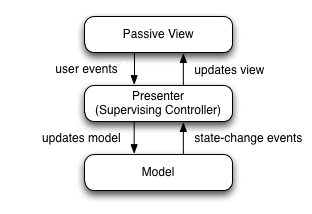
\includegraphics[scale=0.6]{pattern/mvp}
			\caption{Struttura del pattern MVP}
		\label{fig:Struttura_MVP}
	\end{figure}
	
			Model-View-Presenter (MVP) è un pattern architetturale derivato dal MVC (Model-View-Controller), utilizzato per dividere il codice in funzionalità distinte. Il suo principale ambito di utilizzo è nelle applicazioni un insieme di informazioni deve essere rappresentato mediante un'interfaccia grafica.
			\paragraph{Componenti}
			MVC è basato sul principio di disaccoppiamento di tre oggetti distinti, riducendo in questo modo le dipendenze reciproche; inoltre permette di fornire una maggiore modularità, manutenibilità e robustezza al software.
				\subparagraph{Model}
					Il Model rappresenta il cuore dell'applicazione: esso definisce il modello dei dati definendo gli oggetti secondo la logica di utilizzo dell'applicazione, ossia la sua business logic. Inoltre, indica le possibili operazioni che si possono effettuare sui dati.
				\subparagraph{View}
					Nel pattern MVP, il Model è un componente prevalentemente passivo, ma si occupa anche di notificare al Presenter eventuali modifiche del proprio stato. Nella struttura del pattern MVP, la View si occupa di prendere gli input dell'utente e passarli al Controller, affinché esegua operazioni sul Model.
				\subparagraph{Presenter}
					Il Presenter è l'intermediario tra il Model e la View. Si occupa di implementare l'insieme di operazioni eseguibili sul modello dei dati attraverso una particolare vista, ossia l'application logic. Ad ogni View, deve corrispondere un diverso Controller.
				\paragraph{Vantaggi}
					Elenco vantaggi.
				\paragraph{Svantaggi}
					Elenco svantaggi.
			\subsubsection{Dependency injection}
				Dependency injection è un pattern architetturale utilizzato nella programmazione object-oriented al fine di separare il comportamento di una componente dalla risoluzione delle sue dipendenze. Di conseguenza, il pattern su basa su tre elementi:
				\begin{itemize}
					\item un componente dipendente;
					\item la dichiarazione delle dipendenze della componente;
					\item un injector, che crea su richiesta le istanze delle classi che implementano le dipendenze.
				\end{itemize}
				
				Il principio su cui si basa è l'inversione di controllo, secondo il quale il ciclo di vita degli oggetti viene gestito da un'entità esterna, detta container. Nella dependency injection implementata con inversione di controllo, le dipendenze vengono inserite nel container, mentre la componente si limita a dichiararle. In questo modo si limita la dipendenza fra classi. Esistono due tipi di dependency injection:
				
				\begin{description}
					\item[constructor injection:] le dipendenze vengono dichiarate come parametro del costruttore. In questo modo un oggetto è valido appena viene istanziato;
					\item[setter injection:] le dipendenze vengono dichiarate come metodi setter. In questo modo vengono evidenziate le dipendenze.
				\end{description}
				\paragraph{Vantaggi}
					Elenco vantaggi.
				\paragraph{Svantaggi}
					Elenco svantaggi.
	\subsection{Design pattern creazionali}
		\subsubsection{Singleton}
			\begin{figure}[!h]
				\centering
				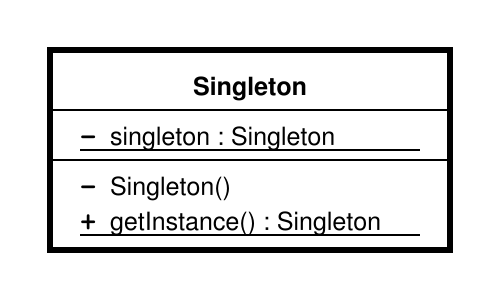
\includegraphics[scale=0.5]{pattern/singleton}
				\caption{Struttura del pattern Singleton}
				\label{fig:Struttura_Singleton}
			\end{figure}
			
			Lo scopo del pattern Singleton è assicurare l'esistenza di un'unica istanza di una classe fornire un punto di accesso globale ad essa. Questo pattern è nate per rispondere alla necessità di non avere più istanza della stessa glasse, pur dando la possibilità alla classe di tener traccia di quella sua istanza. Il pattern Singleton è applicabile ogni volta in cui debba esistere una sola istanza di una determinata classe in tutta l'applicazione, prestando attenzione al fatto che l'istanza sia estendibile tramite ereditarietà.
			\paragraph{Vantaggi}
				Elenco vantaggi.
			\paragraph{Svantaggi}
				Elenco svantaggi.
		\subsubsection{Strategy}
		
			\paragraph{Vantaggi}
				Elenco vantaggi.
			\paragraph{Svantaggi}
				Elenco svantaggi.
	\subsection{Design pattern strutturali}
		\subsubsection{Facade}
			\begin{figure}[!h]
				\centering
				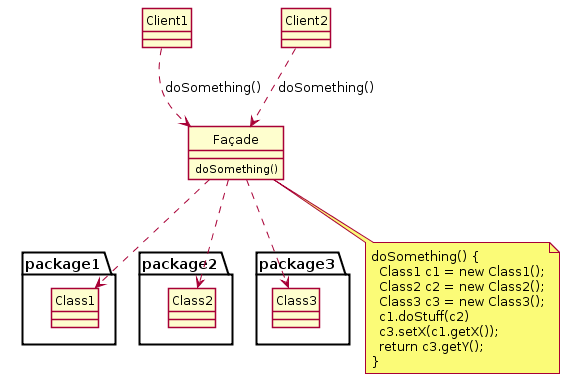
\includegraphics[scale=0.7]{pattern/facade}
				\caption{Struttura del pattern Facade}
				\label{fig:Struttura_Facade}
			\end{figure}		
		
			Lo scopo del pattern strutturale Facade è di fornire un'interfaccia unificata per un insieme di interfacce presenti in un sottosistema, definendo un'interfaccia di livello più alto che rende il sottosistema più semplice da utilizzare. Suddividendo un sistema in sottosistemi, si aiuta a ridurne la complessità e si minimizzano le comunicazioni e le dipendenze fra i diversi sottosistemi.
			\paragraph{Vantaggi}
				Elenco vantaggi.
			\paragraph{Svantaggi}
				Elenco svantaggi.
	\subsection{Design pattern comportamentali}
		\subsubsection{Observer}
			\begin{figure}[!h]
				\centering
				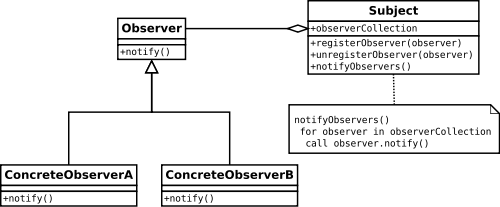
\includegraphics[scale=0.7]{pattern/observer}
				\caption{Struttura del pattern Observer}
				\label{fig:Struttura_Observer}
			\end{figure}
			Observer è un pattern comportamentale il cui scopo è quello di tenere sotto controllo lo stato di diversi oggetti legati ad un soggetto (detta anche \textbf{dipendenza uno a molti}). Il paradigma su cui si basa corrisponde al modello \textbf{Publisher and Subscribe}: i sottoscrittori si registrano presso un pubblicatore e quest'ultimo li informa ogni volta che ci sono nuove notizie. Il pattern è composto da:
				\begin{itemize}
					\item una classe astratta \textbf{Subject} da cui eredita il soggetto concreto, che mantiene una lista di riferimenti agli oggetti dipendenti per poterli avvisare;
					\item un'interfaccia \textbf{Observer} implementata dagli osservatori concreti, che tengono il riferimento al soggetto per poterne leggero lo stato.
				\end{itemize}
			\paragraph{Vantaggi}
				Elenco vantaggi.
			\paragraph{Svantaggi}
				Elenco svantaggi.
\end{document}